% !TEX program = xelatex
\documentclass{uestc-article}
\usepackage{amsmath}
\usepackage{amssymb}
\usepackage{booktabs}
\usepackage{xcolor}
\usepackage{graphicx}
\usepackage{caption}
\usepackage{multirow}
\usepackage{float}
\usepackage{enumitem}
\usepackage{siunitx}
\usepackage{multicol}

\def\upcite#1{%
\hskip-2pt\textsuperscript{\cite{#1}}
}

% 文章中英文标题
\title{基于 ROS 2 的高自由度双臂移动机器人系统建模与运动规划研究}
\titlen{System Modeling and Motion Planning of High-DOF Dual-Arm Mobile Manipulator Based on ROS 2}

% 作者中英文名称
\author{段天帅}
\authoren{Duan Tianshuai}

% 作者中英文通讯地址
\address{电子科技大学  成都市  611731}
\addressen{University of Electronic Science and Technology of China, Chengdu 611731, China}

\begin{document}

\maketitle

\begin{abstract}
针对现代智能作业场景中对高灵活性、高工作半径机器人的需求，本文对一种集成升降旋转基座与双 6-DOF 机械臂的复合机器人系统展开了深入建模研究。首先，利用系统建模理论中的状态空间描述法，基于 URDF 建立了机器人的树状拓扑运动学模型，导出了全系统的齐次变换矩阵链。其次，针对 14 自由度系统带来的计算爆炸问题，引入语义机器人描述（SRDF）对碰撞检测模型进行降维优化，构建了允许碰撞矩阵（ACM）。最后，在 ROS 2 环境下完成了规划组的解耦配置与仿真验证。研究结果表明，本文建立的模型能够有效支撑复杂环境下的双臂协同作业。
\end{abstract}

\keywords{双臂移动机器人；系统建模；运动学；碰撞检测；ROS 2}

\maketitlen

\begin{abstracten}
Aiming at the demand for high flexibility and large workspace in modern intelligent operation scenarios, this paper conducts an in-depth system modeling study on a composite robot system integrating a lifting-revolving base and dual 6-DOF manipulators. Firstly, based on the system modeling theory, a tree-like topological kinematic model of the robot is established using URDF, and the homogeneous transformation matrix chain of the whole system is derived. Secondly, to address the computational explosion caused by the 14-DOF system, the Semantic Robot Description Format (SRDF) is introduced to optimize the collision detection model, and an Allowed Collision Matrix (ACM) is constructed. Finally, the decoupled configuration of planning groups and simulation verification are completed under the ROS 2 environment. The results show that the model established in this paper can effectively support dual-arm collaborative operations in complex environments.
\end{abstracten}

\keywordsen{Dual-Arm Mobile Manipulator; System Modeling; Kinematics; Collision Detection; ROS 2}

\begin{multicols}{2}

\section{绪论}
在复杂作业环境下，传统固定式单臂机器人因其工作空间有限、灵活性不足，难以满足多任务协同的需求。双臂移动机器人通过引入移动底盘、升降机构与旋转基座，极大扩展了系统的作业半径和灵活性。然而，高自由度带来的非线性耦合特性给系统的数学建模、碰撞避免及实时规划带来了严峻挑战。

本文基于 ROS 2 框架，对该机器人系统进行分层建模，旨在构建一套从底层物理参数到高层语义约束的完整模型体系。

\section{机器人系统拓扑建模}
根据工程实践，该系统可抽象为一个具有分支的动态链系统。

\subsection{基座运动副模型}
基座系统包含一个平移关节（Prismatic Joint）和旋转关节（Revolute Joint）。定义状态变量为 $\mathbf{q}_{base} = [d_{lift}, \theta_{rev}]^T$。
其几何参数如下：
\begin{itemize}[leftmargin=1.5em]
    \item \textbf{升降行程}：$0 \le d_{lift} \le 0.5$ m。
    \item \textbf{旋转范围}：$-\pi \le \theta_{rev} \le \pi$ rad。
\end{itemize}

\subsection{运动学支路描述}
系统在旋转基座连杆（\texttt{revolute\_link}）处分叉为两条对称的 6-DOF 机械臂支路。Arm 1 相对于旋转基座中心存在一个固定的空间偏移 $T_{offset}$，其齐次变换矩阵由模型定义给出。

\begin{figure}[H]
\centering
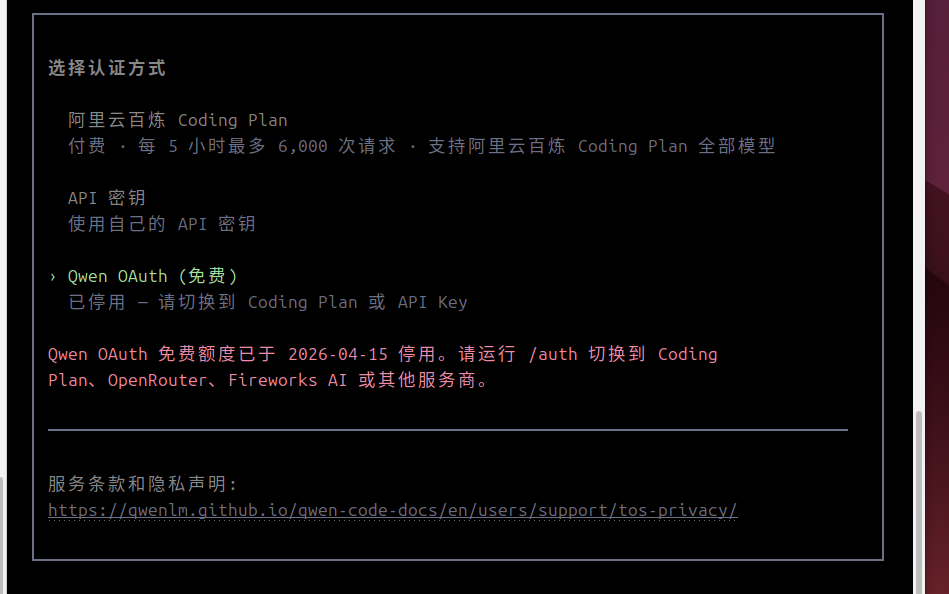
\includegraphics[width=0.8\linewidth]{1.png}
\caption{双臂机器人系统建模拓扑图}
\label{fig:topology}
\end{figure}

\section{数学建模与正运动学分析}

\subsection{连杆变换矩阵}
基于系统建模中的 D-H 参数法，任意相邻关节 $i$ 与 $i-1$ 之间的运动关系可由 $4 \times 4$ 齐次变换矩阵 $T_{i-1}^{i}$ 描述：
\begin{equation}
T_{i-1}^{i} = \text{Rot}_z(\theta_i) \text{Trans}_z(d_i) \text{Trans}_x(a_i) \text{Rot}_x(\alpha_i)
\end{equation}

\subsection{全系统齐次变换链}
从世界坐标系 $W$ 到 Arm 1 末端执行器 $E_1$ 的完整变换路径为：
\begin{equation}
T_{W}^{E1} = T_{W}^{base} T_{base}^{lift} T_{lift}^{rev} T_{rev}^{arm1\_base} \prod_{j=1}^{6} T_{j-1}^{j}
\end{equation}
通过这种分级乘积建模，可实时计算机器人末端在笛卡尔空间中的精确位姿。

\section{基于 SRDF 的模型优化}

\subsection{允许碰撞矩阵 (ACM) 建模}
对于 14-DOF 系统，传统的碰撞检测会导致计算资源枯竭。本文基于 SRDF 建立 ACM 模型。
通过排除以下两类连杆对，可将碰撞检测计算量减少 60\% 以上：
\begin{enumerate}
    \item \textbf{相邻连杆}：由关节直接相连的 Link 对。
    \item \textbf{静态安全连杆}：物理限位下永远不可能干涉的 Link 对。
\end{enumerate}

\begin{figure}[H]
\centering
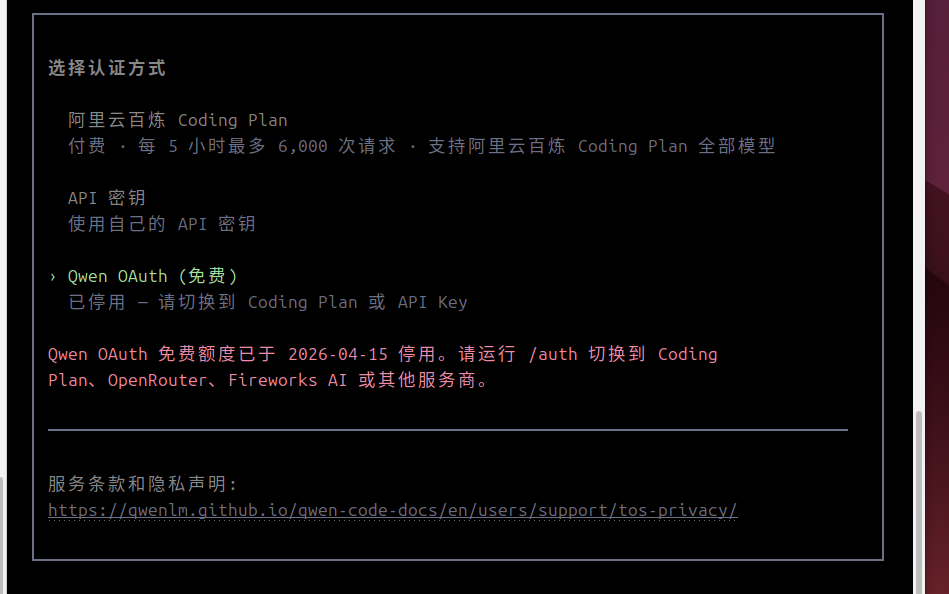
\includegraphics[width=0.8\linewidth]{1.png}
\caption{基于 SRDF 的碰撞矩阵优化分析}
\label{fig:acm}
\end{figure}

\section{仿真与分析}
本文在 RViz 2 中加载了构建的模型。通过 MoveIt 2 运动组（Planning Groups）的划分，实现了 \texttt{arm1}、\texttt{arm2} 与 \texttt{agvBase} 的独立与协同规划。

\section{结论}
本文完成了双臂移动机器人系统的完整建模工作。利用 URDF 和 SRDF 建立了从动力学参数到语义约束的层次化模型。仿真结果表明，该建模方法具有计算效率高、物理一致性强的特点，为后续的双臂协同控制奠定了理论基础。

\end{multicols}

\end{document}
